\documentclass[main.tex]{subfiles}
 
\begin{document}
\chapterimage{band1.jpg}
\chapter{Getting Started}

In this chapter, our aim would be to get our development setup functional, and also to get an understanding for the development tools and repositories available around ESP32.

\section{Development Overview}\index{Development Overview}

The following diagram depicts the typical developer setup for development with ESP.
\begin{figure}[h]
    \centering
    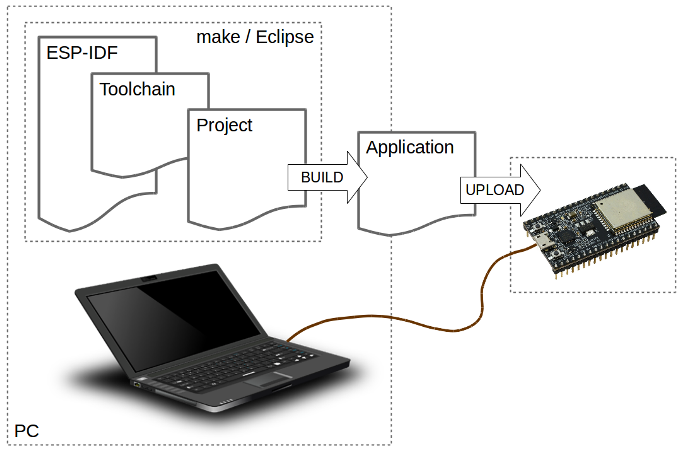
\includegraphics[scale=0.3]{Pictures/dev_setup.png}
    \caption{Typical Developer Setup}
    \label{fig:dev_setup}
\end{figure}

The PC, or the Development Host can be any of Linux, Windows or Mac. The ESP32 based development board is connected to the Development Host over a USB cable. The Development Host has the ESP-IDF (Espressif's SDK), the compiler toolchain and the code for your project. The development host builds this code and generates the executable firmware image. The tools on the Development Host then download the generated firmware image on to the development board. As the firmware executes on the development board, the logs from the firmware can be monitored from the Development Host.

\section{Getting ESP-Jumpstart}\index{Getting ESP-Jumpstart}

Let's get started by cloning the ESP-Jumpstart git repositories \url{https://github.com/espressif/esp-jumpstart}. This repository contains the sequence of applications that we will use for this exercise. This repository also contains a stable release version of IDF as a git submodule. This ensures that we are working off of a stable release of IDF.

\begin{verbatim}
$ git clone --recursive https://github.com/espressif/esp-jumpstart
\end{verbatim}

This repository already contains a copy of the IDF, Espressif's IoT Development Framework. Let's define the IDF\_PATH variable to point to the correction location of IDF. This can be done by executing the following command in your console:

\begin{verbatim}
$ export IDF_PATH=/path/to/esp-jumpstart/esp-idf
\end{verbatim}

Now let's make sure your development host (Windows, Linux or Mac) has the required packages to build and monitor ESP32 based projects. What you specifically need to do is:
\begin{itemize}
    \item Setting the toolchain \url{https://docs.espressif.com/projects/esp-idf/en/latest/get-started/#setup-toolchain}
    \item Establish serial connection with ESP32 \url{https://docs.espressif.com/projects/esp-idf/en/latest/get-started/establish-serial-connection.html}
\end{itemize}

\section{ESP-IDF}\index{ESP-IDF}

ESP-IDF is Espressif's IoT Development Framework. 
\begin{itemize}
    \item ESP-IDF is a collection of libraries and header files that provides the core software components that are required to build any software projects on ESP32. 
    \item ESP-IDF also provides tools and utilities that are required for typical developer and production usecases, like build, flash, debug and measure.
\end{itemize}

The IDF has a component-based design. 

\begin{figure}[h!]
    \centering
    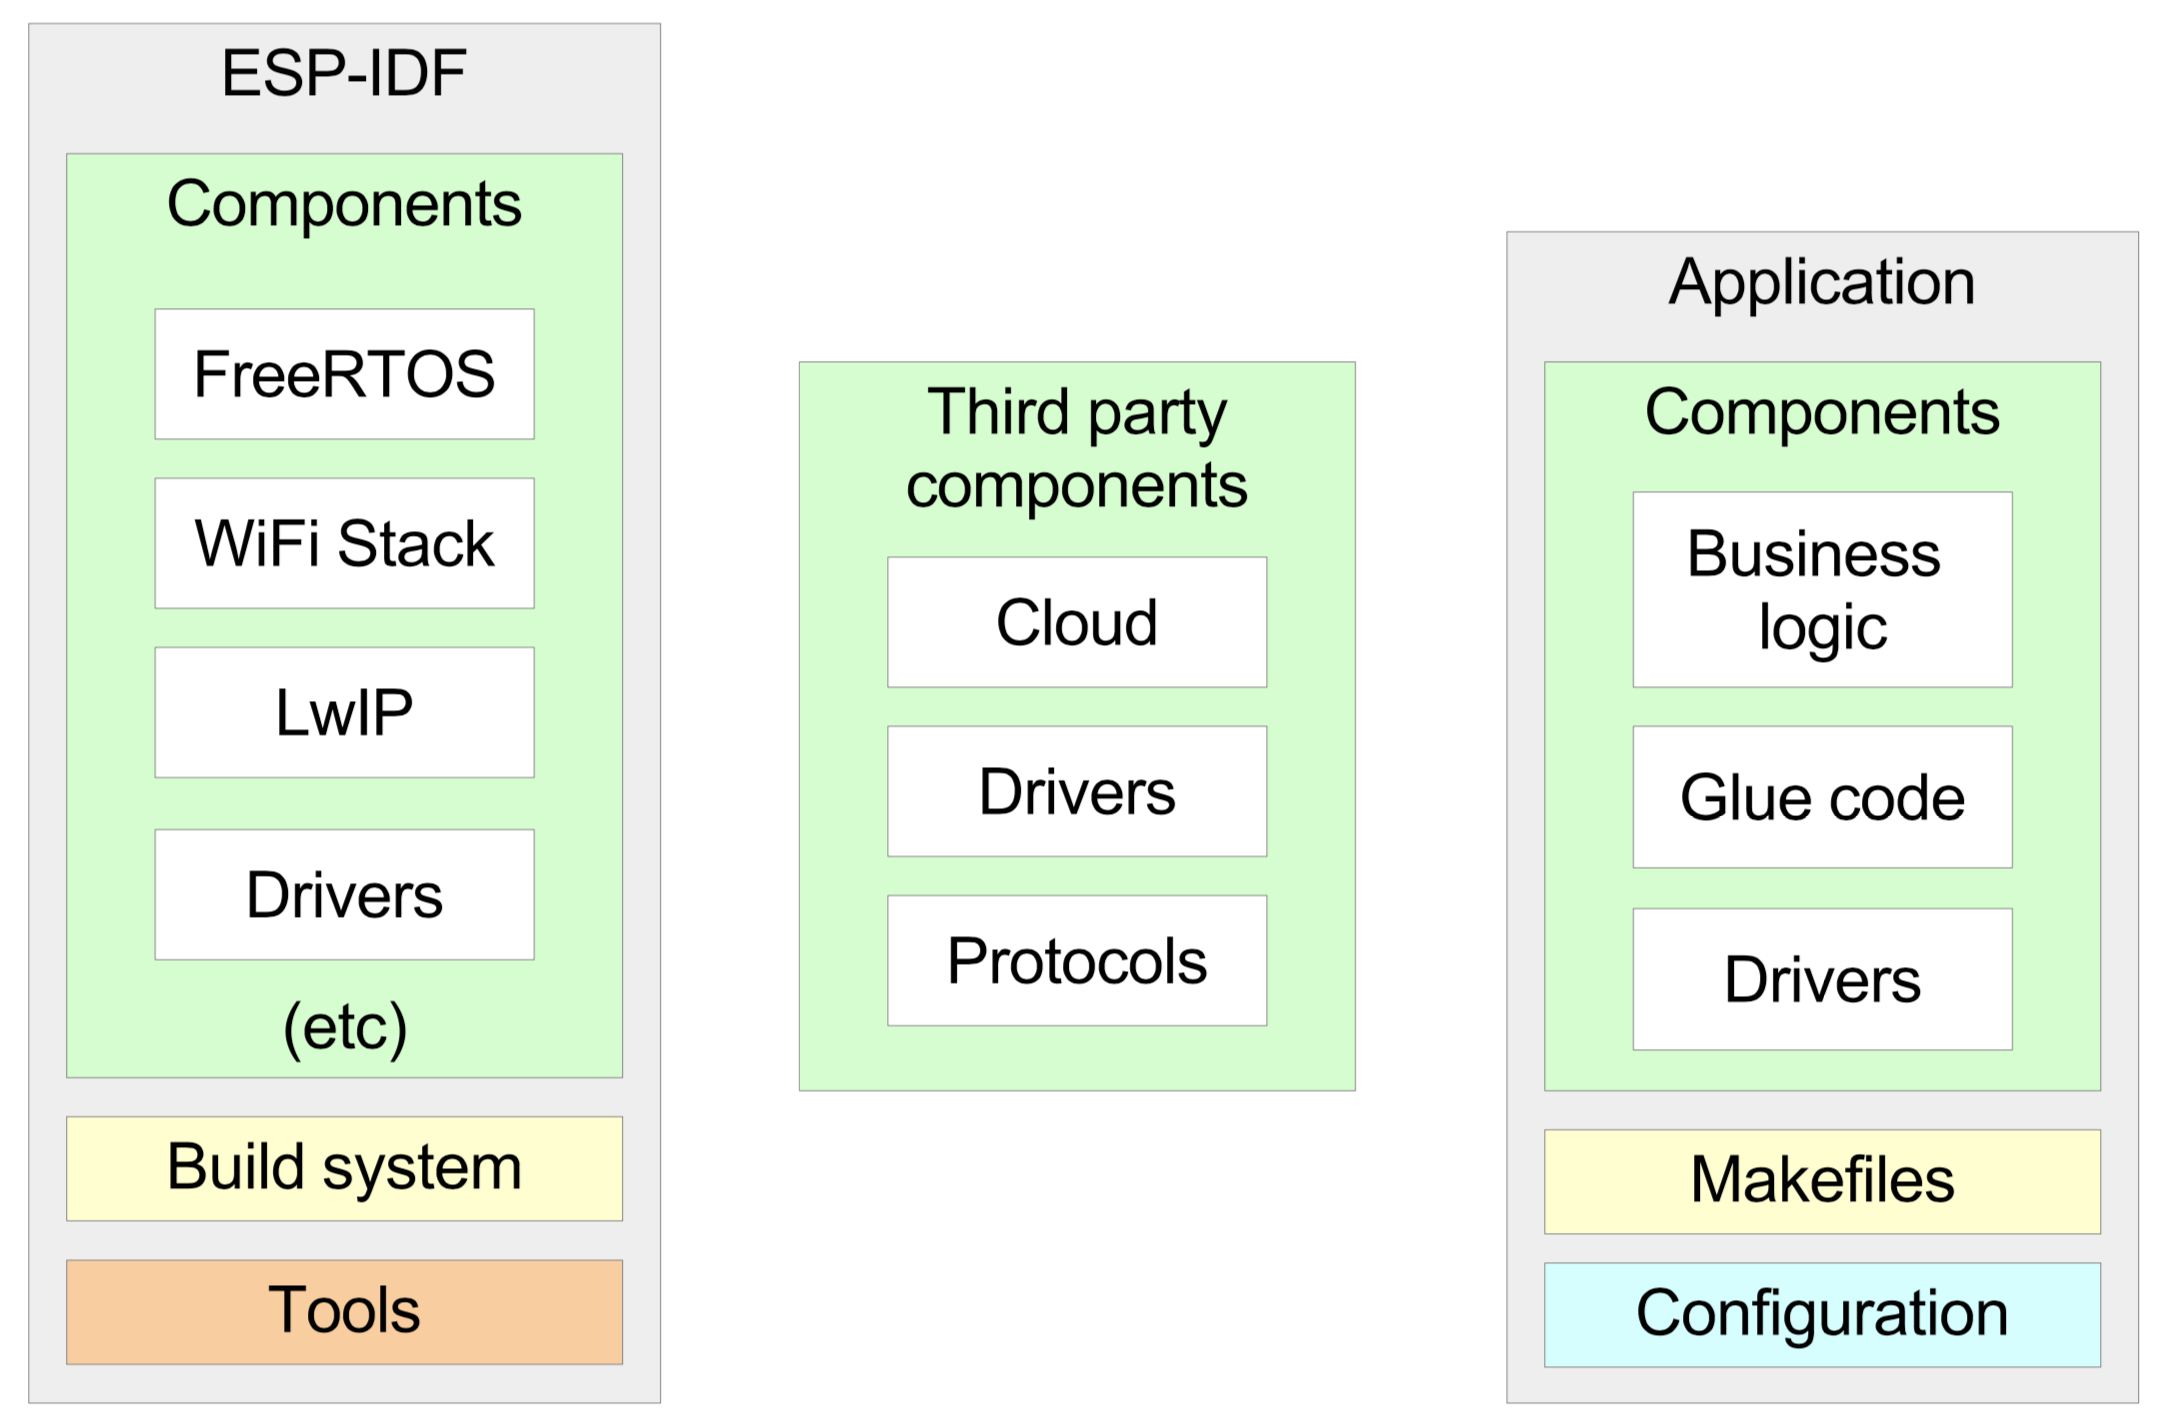
\includegraphics[width=\textwidth]{Pictures/idf_comp.png}
    \caption{Component Based Design}
    \label{fig:idf_comp_design}
\end{figure}

All the software in the IDF is available as components. The Operating System, the network stack, Wi-Fi drivers, middleware modules like the HTTP Server are all components within IDF. 

This design allows you to use your own or third-party components that are built for ESP-IDF.

A developer typically builds \textit{applications} against the IDF. The applications typically contains the business logic, any drivers for externally interfaced peripherals and the SDK configuration.

\begin{figure}[h!]
    \centering
    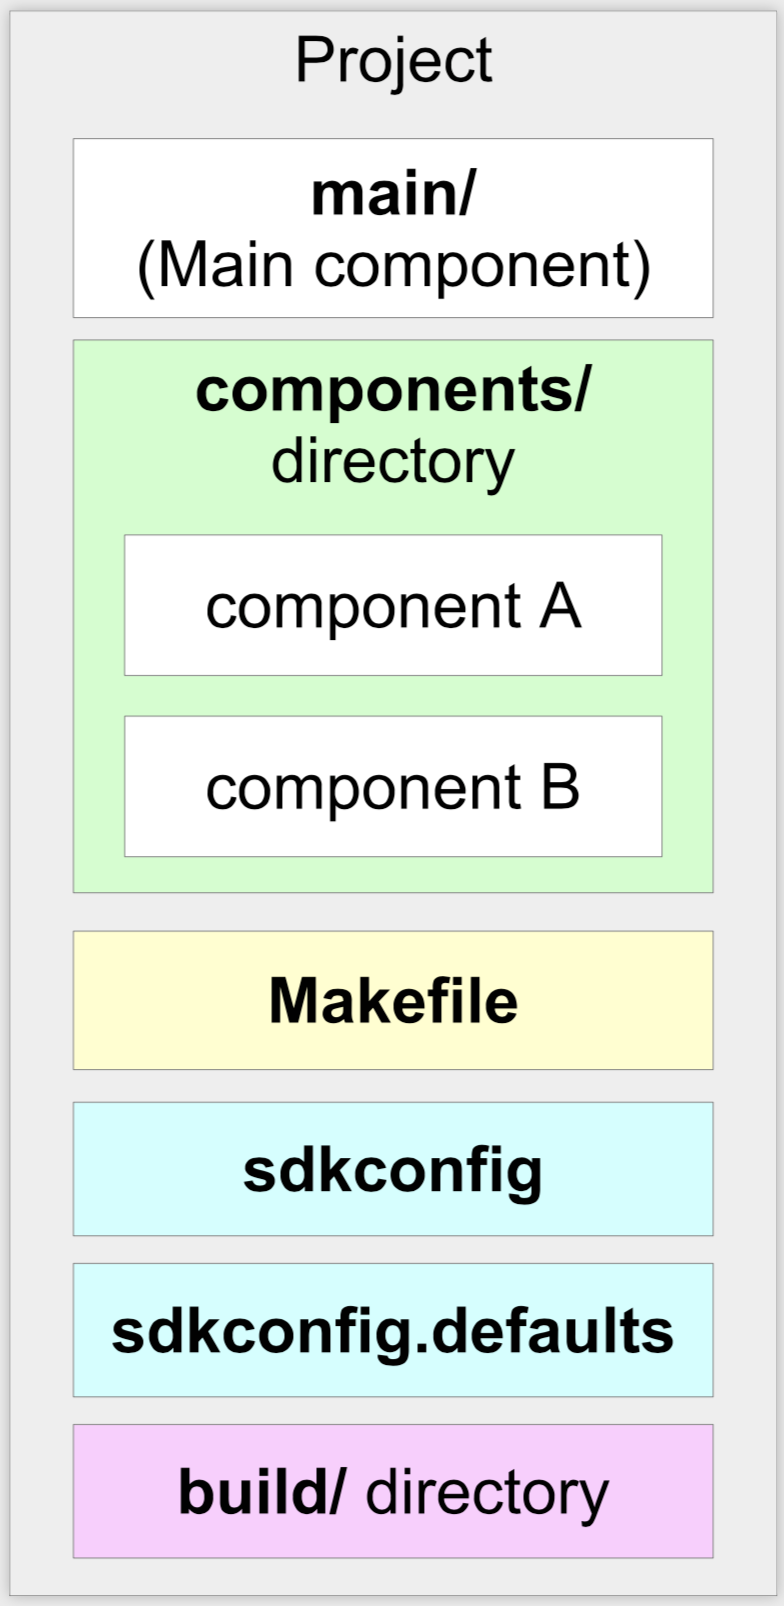
\includegraphics[scale=0.4]{Pictures/app_structure.png}
    \caption{Application's Structure}
    \label{fig:app_structure}
\end{figure}

An application must contain one \textit{main} component. This is the primary component that holds the application logic. The application may additionally include other components as may be desired.
The application's \textit{Makefile} defines the build instructions for the application. 
Additionally, an optional \textit{sdkconfig.defaults} may be placed that picks up the default SDK configuration that should be selected for this application. More details about the SDK configuration follow.

\subsection{SDK Configuration}\index{SDK Configuration}

Given that this is an embedded application with footprint constraints, the IDF allows every application to choose its own SDK configuration. The SDK configuration allows you to select specific configuration options of the SDK that suit your application.

Typically, there is a feature v/s footprint tradeoff, where pulling in a new feature will consume greater memory footprint.

Let us now first use the \textit{Hello World} application and launch the SDK configuration for this application.

\begin{verbatim}
$ cd esp-jumpstart/1_hello_world
$ make -j8 menuconfig
\end{verbatim}

This will first open a pop-up screen for the SDK configuration.

For our current scenario, we will choose the default configuration. Later in this series, we will look at greater details into the SDK configuration options. For now, you can simply exit from this screen. On exiting, when asked for a prompt whether you want to save the SDK configuration, say "Yes".

\ksnotebox{If you are building the application for the first time, the SDK configuration screen will pop-up automatically even if you build for some other build target. For subsequent builds this SDK configuration screen wouldn't show up again unless you specify the \textit{menuconfig} target.}

\subsection{Build and Flash}\index{Build and Flash}
At this point you should have connected the device to your development host. If you have installed the correct drivers, you should see a new device in your machine. For Windows, a new COM port would have been created. For Linux/OSX, a new file would appear in /dev/tty.*. The flashing utility should know which serial port is connected to your device. This can be configured by setting the 'ESPPORT' environment variable. The following command should help:
\begin{verbatim}
$ export ESPPORT=/dev/tty.SLAB_USBTOUART
\end{verbatim}

The rate at which the flashing utility writes firmware to the device can also be configured. This is called the baud rate. The typical rate is 115200. But this can be extended upto 921600. Let's configure the maximum baud rate for our flashing.
\begin{verbatim}
$ export ESPBAUD=921600
\end{verbatim}

Now let's go ahead and ask make to build and flash the firmware.
\begin{verbatim}
$ make -j8 flash monitor
\end{verbatim}

The SDK will then build the entire SDK and the application. Once the build is successful, it will write the generated firmware to the device.

\ksnotebox{On some development boards you may have to press a specific button configuration in order to put the development board into the 'flashing mode'. Please refer to your development board's documentation for these details. For ESP32-DevKit-C, no such button press is required, the board is automatically put into the flashing mode by the flasher utility.}

\section{The Code}\index{The Code}
Now let's look at the code of the Hello World Application. It is only a few lines of code as shown below:
\begin{minted}{c}
#include <stdio.h>
#include "freertos/FreeRTOS.h"
#include "freertos/task.h"


void app_main()
{
    int i = 0;
    while (1) {
        printf("[%d] Hello world!\n", i);
        i++;
        vTaskDelay(5000 / portTICK_PERIOD_MS);
    }
}
\end{minted}
The code is fairly simple. A few takeaways:
\begin{itemize}
\item The app\_main() function is the application entry point. All applications begin execution at this point. This function gets called after the FreeRTOS kernel is already executing on both the cores of the ESP32. Once FreeRTOS is initialis\
ed, it forks an application thread, called the main thread, on one of the cores. The app\_main() function is called in this thread's context. The stack of the application thread can be configured through the SDK configuration.
\item C library functions like printf(), strlen(), time() can be directly called. The IDF uses the newlib C library, which is a low-footprint implementation of the C library. Most of the category of functions of the C library like stdio, stdlib, string operations, math, time/timezones, file/directory operations are supported. Support for signals, locales, wchrs is not available. In our example above, we use the printf() function for printing to the console.
\item FreeRTOS is the operating system powering both the cores. FreeRTOS (https://www.freertos.org) is a tiny kernel that provides mechanisms for task creation, inter-task communication (sempahores, message queues, mutexes), interrupts and timers. In our example above, we use the vTaskDelay function for putting the thread to sleep for 5 seconds. Details of the FreeRTOS APIs are available at: https://www.freertos.org/a00106.html
\end{itemize}

\section{Progress so far}\index{Progress so far}
Now we have the basic development setup and process in place. We can build the code into executable firmware images. We can flash these images to a connected development board, and we can monitor the console to look at debug logs and messages generated by the firmware. 

Let's now build a simple power outlet with ESP32.

\end{document}
